\documentclass[14pt, a4paper]{extreport}

\usepackage{susu}

% ====================================================================================================
\begin{document}

\author{Олейников~Е.О.}
\group{212}
\task{1}
\maketitle

% ====================================================================================================
\chapter{Задание}

\begin{enumerate}

	\item
	Разработать подпрограммы для градиентной закраски прямоугольной области различными способами.
	Аргументы подпрограмм -- координаты левого верхнего угла, ширина и высота области.
	Подпрограммы должны работать для любого соотношения размеров прямоугольной области.
	Для каждого способа закраски определить зависимость интенсивности цвета от координат точки.
	При реализации подпрограмм использовать для рисования только процедуру putpixel.

	\item
	Написать программу для тестирования разработанных \linebreak подпрограмм.
	Интерфейс программы должен содержать следующие элементы управления:
	\begin{itemize}
		\item выбор способа закраски;
		\item сохранение результата в файл;
		\item выход из программы.
	\end{itemize}

\end{enumerate}

% ====================================================================================================
\chapter{Математическая модель}

Пусть $x_0$, $y_0$, $w$, $h$ -- соответственно координаты левого верхнего угла, ширина и высота прямоугольной области.
При закрашивании выполняется обход всех точек области.
Цвет точки $(x;y)$ задается в цветовой модели RGB.
Значения интенсивностей равны 0, $\frac{c}{2}$ и $c$ соответственно для красной, зеленой и синей составляющей цвета.
Максимальное значение интенсивности $c_{max} = 255$.
Переменная $c$, определяющая интенсивность составляющих цвета, вычисляется в соответствии с приведенными ниже формулами.

Способ~1. Интенсивность цвета зависит только от ординаты точки:
$$ c = \frac{y - y_0}{h} c_{max} . $$

Способ~7. Интенсивность цвета зависит от расстояния от точки до центра прямоугольной области:
$$ c = \left\{ \begin{aligned} (1 - d) c_{max} &, d < 1; \\ 0 &, d \geq 1, \end{aligned} \right. $$
где
$$ d = \frac{1}{r} \sqrt{\left( x - x_0 - \frac{w}{2} \right) ^ 2 + \left( y - y_0 - \frac{h}{2} \right) ^ 2}, $$
$$ r = \left\{ \begin{aligned} \frac{w}{2} \ &, w < h; \\ \frac{h}{2} \ &, w \geq h. \end{aligned} \right. $$

% ====================================================================================================
\chapter{Текст программы}

\noindent Файл main.cpp
\lstinputlisting{source/main.cpp}
\pagebreak
\hrulefill

\noindent Файл task.h
\lstinputlisting{source/task.h}
\hrulefill

\noindent Файл task.cpp
\lstinputlisting{source/task.cpp}
\hrulefill

\noindent Файл control.h
\lstinputlisting{source/control.h}
\hrulefill

\noindent Файл control.cpp
\lstinputlisting{source/control.cpp}

% ====================================================================================================
\chapter{Результат работы}

\begin{figure}[h!]
	\centering
	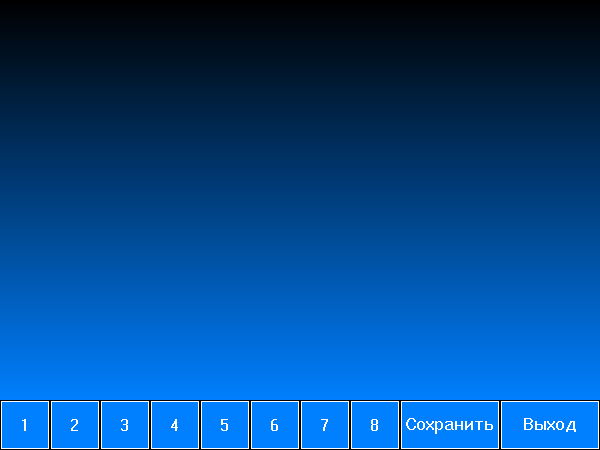
\includegraphics[width = 12cm]{image/image_1}
  \caption{Результат выполнения программы (способ 1)}
\end{figure}

\begin{figure}[h!]
	\centering
	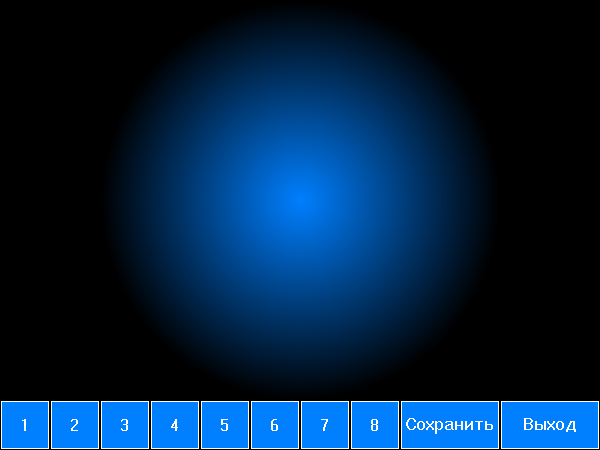
\includegraphics[width = 12cm]{image/image_7}
  \caption{Результат выполнения программы (способ 7)}
\end{figure}

% ====================================================================================================
\end{document}